

\begin{frame}{Do czego potrzebna jest mapa}
	Możliwa jest nawigacja bez wykorzystania mapy, w tym wypadku wykorzystuje się tak zwaną nawigację zliczeniową. 
	Jej wykorzystanie powoduje akumulację błędu pozycji, którego nie da się zniwelować,
	a który rośnie z czasem.
	Dlatego potrzebne są punkty orientacyjne, które pozwalają utrzymać błąd lokalizacji w pewnych granicach \cite{robotics_vision_dead_reckon}.
\end{frame}

\begin{frame}{Jak działa budowa mapy}
	\begin{itemize}
		\item początkowe założenie - znana pierwotna pozycja robota
		\item uzyskanie punktów otoczenia względem robota
		\item możliwośc wykorzystania wielu czujników - systemu LiDAR, kamery Kinect, sonarów etc.
		\item możliwość identyfikowania poszczególnych punktów na mapie aby moć je od razu rozpoznać lub przechowywanie jedynie współrzędnych zajętych obszarów
	\end{itemize}
\end{frame}

\begin{frame}{Jak działa budowa mapy}
	\begin{columns}
		\begin{column}{0.5\textwidth}
			\begin{figure}
				\centering
				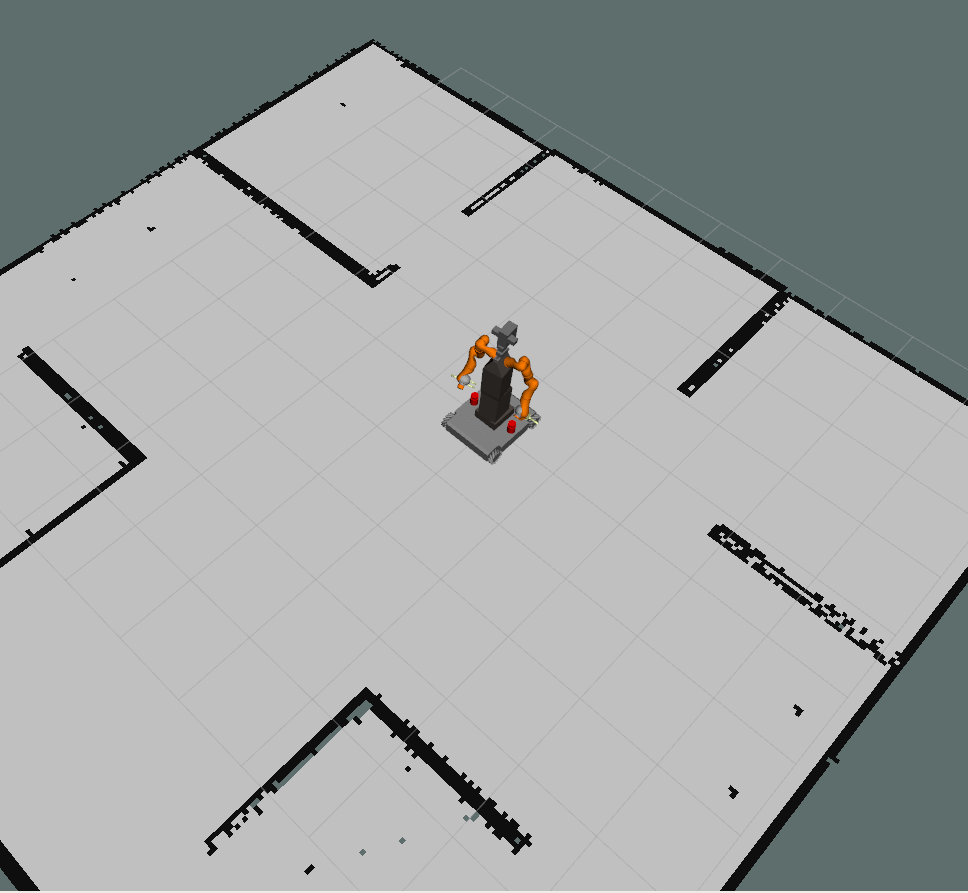
\includegraphics[height=0.6\textheight]{img/mapa_2d.png}
				\caption{dwuwymiarowa mapa zbudowana przy pomocy czujników LiDAR}
			\end{figure}
		\end{column}
		\begin{column}{0.5\textwidth}  %%<--- here
			\begin{figure}
				\centering
				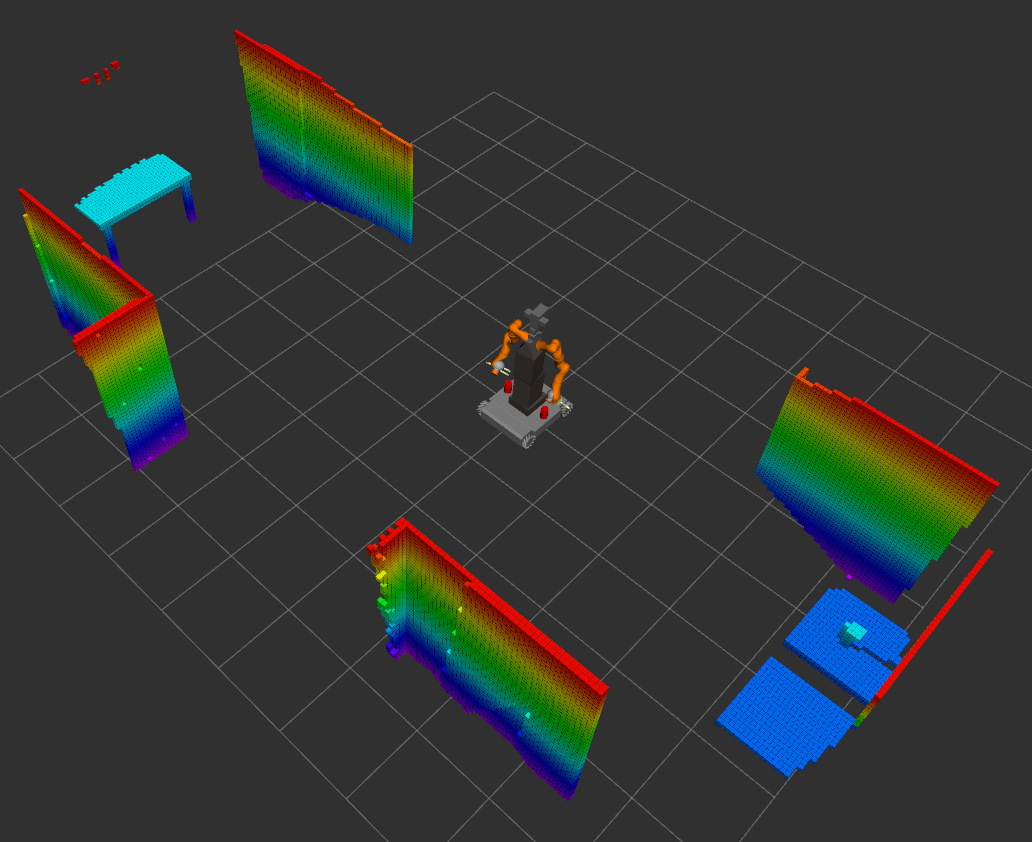
\includegraphics[height=0.6\textheight]{img/octomapa.png}
				\caption{mapa trójwymiarowa zbudowana przy pomocy kamery Kinect}
			\end{figure}
		\end{column}
	\end{columns}
\end{frame}

\begin{frame}{Własności niektórych metod}
	\begin{columns}
		\begin{column}{0.5\textwidth}
			\begin{center}
				czujnik LiDAR
			\end{center}
			\begin{itemize}
				\item szybkie tworzenie obrazów dużych płaskich przestrzeni
				\item informacje pobrane tylko na jednej wysokości, zwykle blisko podłoża (mapa 2D)
			\end{itemize}
		\end{column}
		\begin{column}{0.5\textwidth}  %%<--- here
			\begin{center}
				kamera Kinect
			\end{center}
			\begin{itemize}
				\item mniejszy kąt widzenia czujnika i większe nakłady obliczeniowe - potrzeba więcej zasobów do budowy takiej mapy				
				\item budowa obrazu trójwymiarowej przestrzeni
			\end{itemize}
		\end{column}
	\end{columns}
\end{frame}
